\chapter[Anexos]{Anexos}
\label{chap:anexos}

	\section[Anexo A]{\emph{Anexo A - Cálculo do Dimensionamento de Condutores}}
	\label{sec:anexoA}

		\begin{figure}[!h]
			\centering
			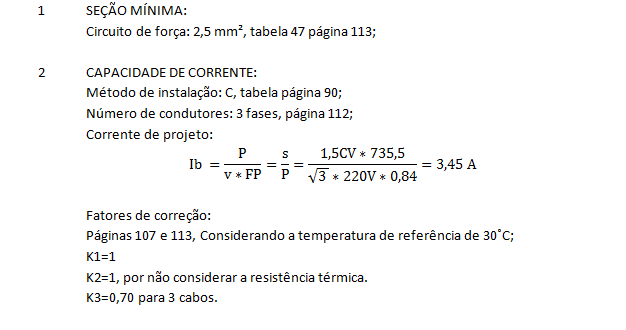
\includegraphics[scale=1]{AnexoA01.png}
			\caption{Anexo A - Parte I} 
			\label{AnexoA01}
		\end{figure}

		\newpage
		\begin{figure}[!h]
			\centering
			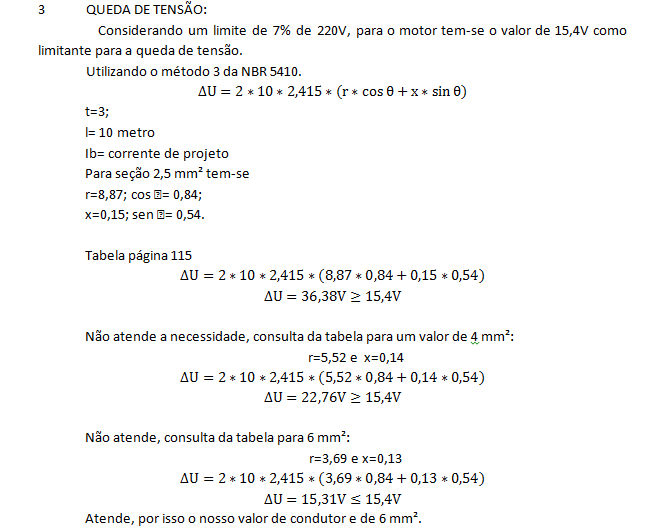
\includegraphics[scale=1]{AnexoA02.png}
			\caption{Anexo A - Parte II} 
			\label{AnexoA02}
		\end{figure}

		\newpage
		\begin{figure}[!h]
			\centering
			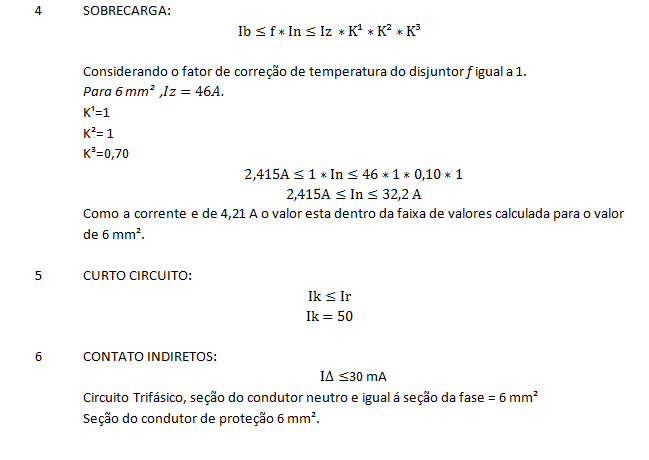
\includegraphics[scale=1]{AnexoA03.png}
			\caption{Anexo A - Parte III} 
			\label{AnexoA03}
		\end{figure}

	\newpage
	\section[Anexo B]{\emph{Anexo B - Programação dos Parâmetros no Inversor de Frequência para Variação das Velociades pelas Chaves Seletoras}}
	\label{sec:anexoB}

		O inversor foi programado para os seguintes parâmetros:

		\begin{itemize}
			\item Parâmetro P000 com o valor 5, liberando a programação do inversor;
			\item Parâmetro P204 com o valor 5, carregando as configurações de fábrica do inversor com dos equipamentos conectados de frequência de 60Hz;
			\item Novamente o parâmetro P000 com o valor 5;
			\item O parâmetro P220 com o valor 0;
			\item O parâmetro P221 com o valor 8;
			\item Parâmetro P223 com o valor 2;
			\item Parâmetro P224 com o valor 1, configurando assim a função multispeed;
			\item Para a configuração das velocidades, parâmetro P124 com o valor 200;
			\item Parâmetro P125 com o valor de 600;
			\item Parâmetro P126 com 1200;
			\item Parâmetro P127 com o valor de 1700;
		\end{itemize}

	\newpage
	\section[Anexo C]{\emph{Anexo C - Dimensionamento Técnico de Condutores e Dispositivos de Proteção}}
	\label{sec:anexoC}

		Dimensionamento técnico de condutores e respectivo dispositivos de proteção, conforme NBR 5410:2004, em anexo os cálculos utilizando os seis critérios que a norma trata:

		\begin{itemize}
			\item Capacidade de condução de corrente;
			\item Queda de tensão;
			\item Seção mínima;
			\item Sobrecarga;
			\item Curto-circuito.
		\end{itemize}

		Para que um circuito esteja dimensionado de forma correta é necessário aplicar seis critérios, sendo que o resultado de cada seção é aplicado a cada um dos critérios, sendo considerado o de maior seção dentre eles para implementação \cite{NBR5410}.
		
		O primeiro critério aplicado foi o de seção mínima, que foi determinada levando em consideração a NBR 5410:204, como circuito de força. A segunda seção refere-se à capacidade de corrente, feita o cálculo de corrente de projeto com valor obtido de 3,45 A, com fatores de correção aplicados, a secção mínima inicialmente foi de 2,5 $mm^{2}$ \cite{NBR5410}.
		
		Utilizando o critério de queda de tensão com limite de 7\% para 220V, considerando como valor limitante de 15,4V, foi possível calcular o novo valor de diâmetro do condutor como 6$mm^{2}$. Aplicando os demais critérios de sobrecarga e curto-circuito o valor permaneceu de 6$mm^{2}$, para o condutor no acionamento no motor de indução trifásica que será utilizado \cite{NBR5410}.

		\textbf{Dispositivos de Proteção}

		O fusível utilizado para a partida de motor é do tipo D- Diazed, Indicado para circuitos de acionamento de motores, pois possui corrente de ruptura de até 17 KA, faixa de corrente que suporta é entre 2 a 63A, tem função retardada, ou seja, suporta a corrente de pico do motor antes de romper, e indicação de corrente que o filamento suporta \cite{WEG04}. Para instalação de um fusível em um circuito elétrico, é necessário componente para sua fixação, o próprio fusível, tampa, parafuso de ajuste, anel de proteção e base \cite{WEG04}.
		
		O dimensionamento de fusível é possível, levando em consideração, a corrente de partida como sendo a razão de corrente de partida pela correte nominal, disponível na placa de identificação do motor, que multiplicada pela corrente nominal, esse valor obtido é de 26,35 A. Porém esse dado não é suficiente para determinar o fusível que será utilizado \cite{WEG04}.
		
		Para a partida direta utiliza-se em geral o tempo de 5 segundos que é associado ao tempo necessário para que o motor saia de sua inércia e atinja a sua velocidade nominal, característica que está associada ao tipo de acionamento do motor escolhida. Portanto, para o valor de fusível, foi dimensionado o de 6 A , porém como na partida será utilizando um inversor de frequência com corrente de 6 A, o valor calculado foi de 16 A \cite{WEG04} \cite{NBR5410}.


	\newpage
	\section[Anexo D]{\emph{Anexo D - Considerações sobre a Temperatura de Operação do Motor de Indução}}
	\label{sec:anexoD}

		A vida útil do motor de indução depende quase que exclusivamente da isolação dos enrolamentos. A isolação é afetada por fatores como umidade, vibrações, ambientes corrosivos e outros. O fator mais importante é a temperatura dos materiais isolantes empregados. Um aumento entre 8 $^{\circ}C$ e 10 $^{\circ}C$ na temperatura de isolação pode reduzir a vida útil do motor pela metade \cite{Goncalez}. A experiência com motores de indução mostra que a isolação tem um tempo de duração praticamente ilimitado, se a sua temperatura for mantida abaixo de certo limite. Acima deste valor, a vida útil da isolação vai se tornando cada vez mais curta, à medida que a temperatura de trabalho é mais alta \cite{Goncalez}. Esta limitação refere-se ao ponto mais quente da isolação e não do enrolamento como um todo.
	
		Os motores de indução possuem uma classe de isolamento com determinados limites de temperatura para a operação. O motor de indução utilizado na bancada de testes para amortecedores possui uma classe de isolação F \cite{Voges}. Para esta classe de isolação, o limite de temperatura para o trabalho é de 155 $^{\circ}C$, conforme mostra a figura abaixo, e, com esta temperatura de operação, sua vida será de 90.000 horas \cite{ABNT17094}.

		\begin{figure}[!h]
			\centering
			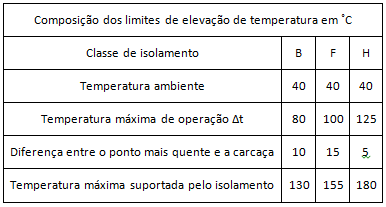
\includegraphics[scale=1]{classeMotor.png}
			\caption[Classes do motor de elevação de temperatura conforme NBR 17094:2003]{Classes do motor de elevação de temperatura conforme \cite{ABNT17094}} 
			\label{classeMotor}
		\end{figure}

		O controle de temperatura é difícil de se obter por intermédio de sensores de temperatura e termômetros, pois não há uma relação linear de variação nos enrolamentos, sendo impossível identificar onde está o ponto mais quente do motor. Por isso, é utilizado o método de variação da sua resistência ôhmica em ensaio, que aproveita a propriedade dos condutores de variar sua resistência \cite{WEG05}. O cálculo é feito com através da equação:

		$$ D_{t} = t_{2} - t_{a} = (\frac{R_{2} - R_{1}}{R_{1}}) * (235 + t_{1}) + (t_{1} - t_{a}) $$

		Onde:
		\begin{itemize}
			\item $D_{t}$ = Elevação de temperatura;
			\item $t_{2}$ = Temperatura dos enrolamentos no fim do ensaio;
			\item $t_{a}$ = Temperatura do meio refrigerante no fim do ensaio;
			\item $t_{1}$ = Temperatura do enrolamento antes ensaio;
			\item $R_{1}$ = Resistência antes do ensaio;
			\item $R_{2}$ = Resistência do enrolamento no fim do ensaio.
		\end{itemize}

		Durante os testes na bancada, é recomendado que o motor opere abaixo do limite de 155 $^{\circ}C$, para que assim não haja redução na vida útil da isolação do motor. Diante dos testes executados com o motor, os quais duraram cerca de 8 minutos de funcionamento contínuo em diferentes velocidades, e do tempo previsto de operação do motor durante o teste real de amortecedores (que depende do tipo de teste realizado) foi possível notar que a variação na temperatura externa do motor foi baixa.  

